%----------------------------------------------------------------------------------------
% GEGEVENS ANALYSEREN. Alle opgaven zijn eigen werk; alle gegevens zijn verzonnen.
%
% Opbouw: Probleem, Start, leerstof, en op een nieuwe pagina de Opdrachten en Test jezelf (geen Koppel in de 2de graad).
% Labels van dit hoofdstuk beginnen met h3-.
% Verschillen per pakket: de regel van 1,5 keer de interkwartielafstand voor uitschieters, met de aangepaste boxplot (4-5).
%----------------------------------------------------------------------------------------

\mychapter{3}{Gegevens analyseren}

\begin{probleem}
Een gemeente telt elk jaar hoeveel fietsers er gemiddeld per dag door de hoofdstraat rijden (verzonnen gegevens): 1820 in 2019, 1850 in 2020, 1870 in 2021, 1890 in 2022, 1910 in 2023 en 1960 in 2024. Het gemeentebestuur toont grafiek 1 en zegt: \textit{Het aantal fietsers is spectaculair gestegen.} De oppositie toont grafiek 2 en zegt: \textit{Het aantal fietsers is nauwelijks veranderd.}

\figuren{\begin{tikzpicture}[x=.72cm,y=.02cm,font=\scriptsize]
  \foreach \t in {50,100,150}{\draw[black!12] (-.6,\t) -- (5.6,\t); \pgfmathtruncatemacro{\l}{1800+\t}\node[left] at (-.6,\t) {\l};}
  \node[left] at (-.6,0) {1800};
  \draw[->,grijs] (-.6,0) -- (-.6,185);
  \draw[grijs] (-.6,0) -- (5.6,0);
  \foreach \v [count=\i from 0] in {1820,1850,1870,1890,1910,1960}{\staaf{\i}{\v-1800}{.55} \pgfmathtruncatemacro{\j}{2019+\i}\node[below] at (\i,0) {\j};}
  \node at (2.5,-30) {grafiek 1};
\end{tikzpicture}\qquad\qquad
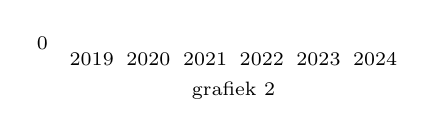
\begin{tikzpicture}[x=.72cm,y=.0016cm,font=\scriptsize]
  \frequentieas[fietsers per dag]{500}{2000}{-.6}{5.6}
  \node[left] at (-.6,0) {0};
  \foreach \v [count=\i from 0] in {1820,1850,1870,1890,1910,1960}{\staaf{\i}{\v}{.55} \pgfmathtruncatemacro{\j}{2019+\i}\node[below] at (\i,0) {\j};}
  \node at (2.5,-375) {grafiek 2};
\end{tikzpicture}}

Allebei de grafieken tonen dezelfde getallen. Hoe kan de ene zo'n grote stijging tonen, en de andere bijna niets? Wie heeft gelijk?
\end{probleem}

\lkr{Leerplan \pakketnaam: LPD \alleenvoor{1}{27-29}\alleenvoor{2}{31-33}\alleenvoor{3}{33-35}\alleenvoor{4,5}{37-39} (dit hoofdstuk: de vorm van een verdeling, uitschieters, groepen vergelijken, een gepaste maat kiezen en misleidende grafieken herkennen). Welk doel bij welk hoofdstuk hoort, is na te kijken in het leerplan. Steekproeven, bias en het verschil tussen samenhang en oorzaak komen in de 3de graad uitgebreid aan bod; hier blijft het bij een kritische blik op grafieken en conclusies. \alleenvoor{4,5}{De regel van 1,5 keer de interkwartielafstand en de aangepaste boxplot staan alleen in pakket 4 en 5.}\alleenvoor{1,2,3}{Uitschieters worden hier op het zicht herkend; de regel van 1,5 keer de interkwartielafstand staat in pakket 4 en 5.} Laat leerlingen hun conclusies altijd in volzinnen en in de context formuleren.}

Je kunt nu gegevens voorstellen en samenvatten. Maar wat zeggen ze? In dit hoofdstuk leer je de vorm van een verdeling beschrijven, groepen vergelijken, en kiezen welke maat bij welke gegevens past. Op het einde kijk je kritisch naar grafieken: met dezelfde getallen kun je een heel ander verhaal vertellen, zoals het probleem toont.

\begin{oefeningen}[Start]
\oef{h3-start-1}

\oef{h3-verken}
\end{oefeningen}

%========================================================================================
\section{De vorm van een verdeling}

\subsection{Symmetrisch en scheef}

Het histogram van de schermtijden in hoofdstuk 1 was hoog aan de linkerkant en liep naar rechts langzaam af. Bij de lengtes van leerlingen zie je eerder een berg in het midden, die aan beide kanten even snel daalt. En bij een gemakkelijke toets halen de meeste leerlingen hoge punten, met enkele uitzonderingen naar onder. De vorm van een histogram zegt dus iets over de gegevens. Die vormen krijgen een naam.

\begin{theorie}
Een verdeling is \textbf{\textcolor{accent}{symmetrisch}} als het histogram links en rechts van het midden ongeveer elkaars spiegelbeeld is.

\vspace{1mm}
Een verdeling is \textbf{\textcolor{accent}{rechtsscheef}} als het histogram een lange staart naar rechts heeft, en \textbf{\textcolor{accent}{linksscheef}} als het een lange staart naar links heeft.

\figuren{\begin{tikzpicture}[x=.3cm,y=.15cm,font=\scriptsize]
  \foreach \a/\f in {0/2,2/5,4/9,6/9,8/5,10/2}{\balk{\a}{\a+2}{\f}} \draw[grijs] (0,0) -- (12,0); \node at (6,-2.2) {symmetrisch};
  \begin{scope}[xshift=5.2cm]\foreach \a/\f in {0/5,2/10,4/7,6/4,8/2,10/1}{\balk{\a}{\a+2}{\f}} \draw[grijs] (0,0) -- (12,0); \node at (6,-2.2) {rechtsscheef};\end{scope}
  \begin{scope}[xshift=10.4cm]\foreach \a/\f in {0/1,2/2,4/4,6/7,8/10,10/5}{\balk{\a}{\a+2}{\f}} \draw[grijs] (0,0) -- (12,0); \node at (6,-2.2) {linksscheef};\end{scope}
\end{tikzpicture}}
\end{theorie}

Let op de namen: de staart bepaalt de naam, niet de top. Een rechtsscheve verdeling heeft haar top links, en haar staart rechts. Bij een boxplot zie je de vorm ook: bij een rechtsscheve verdeling is de rechtersnorhaar lang, en ligt de mediaan in de linkerhelft van de box.

\voorbeeld{}{Beschrijf de vorm van de verdeling van de schermtijden uit hoofdstuk 1, met het histogram en de boxplot.\label{vb:h3-vorm}}{%
\uitleg{We kijken waar het histogram het hoogst is en aan welke kant de staart langer is. Daarna controleren we met de boxplot.}
\figuren{\begin{tikzpicture}[x=.022cm,y=.15cm,font=\scriptsize]
  \foreach \a/\f in {50/7,100/11,150/10,200/7,250/3,300/2}{\balk{\a}{\a+50}{\f}}
  \draw[grijs] (50,0) -- (350,0);
  \foreach \a in {50,150,250,350}{\node[below] at (\a,0) {\a};}
\end{tikzpicture}\qquad
\begin{tikzpicture}[x=.022cm,font=\scriptsize]
  \boxplot{.7}{58}{108.5}{158}{216}{319}
  \getalas[min]{50}{100}{350}
\end{tikzpicture}}
Het histogram is het hoogst bij 100 tot 200 minuten en heeft een lange staart naar rechts: de verdeling is rechtsscheef. In de boxplot is de rechtersnorhaar ($319 - 216 = 103$) twee keer zo lang als de linker ($108,5 - 58 = 50,5$). Veel leerlingen zitten één tot drie uur op hun smartphone, enkelen veel langer.}

\begin{oefeningen}
\oef{h3-vorm}
\end{oefeningen}

\subsection{Gemiddelde en mediaan}

In hoofdstuk 2 zagen we dat een uitschieter het gemiddelde meetrekt, maar de mediaan niet. Een staart is een hele groep gegevens aan één kant. Wat doet die met het gemiddelde? Bij de schermtijden is de mediaan 158 minuten en het gemiddelde ongeveer 165,6 minuten: het gemiddelde ligt rechts van de mediaan, aan de kant van de staart.

\begin{theorie}
\begin{stelling}{Gemiddelde en mediaan}
Bij een \textbf{\textcolor{accent}{rechtsscheve}} verdeling is meestal $\formule{\xbar > \Me}$. Bij een \textbf{\textcolor{accent}{linksscheve}} verdeling is meestal $\formule{\xbar < \Me}$. Bij een symmetrische verdeling is $\formule{\xbar \approx \Me}$.
\end{stelling}
\end{theorie}

Het woord \textit{meestal} staat er bewust: het is een vuistregel, geen wet. Je kunt rijen gegevens bedenken die er niet aan voldoen. Toch is de regel handig: vergelijk je het gemiddelde met de mediaan, dan weet je iets over de vorm zonder het histogram te zien.

\voorbeeld{}{Twintig leerlingen maken een gemakkelijke toets op 20. Hun punten zijn: 18, 17, 19, 16, 18, 20, 15, 17, 19, 18, 12, 16, 19, 17, 18, 9, 18, 19, 17, 16. Bereken het gemiddelde en de mediaan. Wat zegt dat over de vorm?\label{vb:h3-gemmed}}{%
\uitleg{We berekenen beide centrummaten en kijken welke groter is.}
\begin{stappenbreed}
\xbar = \dfrac{338}{20} = 16,9 & De som van de punten is 338. \\[2ex]
9,\ 12,\ 15,\ 16,\ \dots,\ 17,\ \fbox{17},\ \fbox{18},\ 18,\ \dots,\ 20 \qquad \Me = 17,5 & Het 10de en het 11de getal zijn 17 en 18. \\
\xbar = 16,9 < 17,5 = \Me & Het gemiddelde ligt links van de mediaan.
\end{stappenbreed}
De verdeling is linksscheef: de meeste leerlingen halen 16 tot 20, maar de punten 9 en 12 vormen een staart naar links. Die trekken het gemiddelde naar beneden.}

\begin{oefeningen}
\oef{h3-gemmed}
\end{oefeningen}

\subsection{Uitschieters}

Een uitschieter is een gegeven dat ver van de andere ligt. Het kan een meetfout of tikfout zijn, maar ook een echte, uitzonderlijke waarde. Je mag een uitschieter dus niet zomaar weglaten: zoek eerst uit waar hij vandaan komt.

\voorbeeld{}{Twaalf leerlingen meten hun reactietijd (in s) met een app: 0,31; 0,28; 0,35; 0,30; 0,33; 0,29; 0,32; 0,34; 0,27; 0,31; 0,30; 0,62. Welk gegeven is een uitschieter? Wat is zijn invloed op het gemiddelde, de mediaan en de standaardafwijking?\label{vb:h3-uitschieter}}{%
\uitleg{Alle tijden liggen tussen 0,27 en 0,35 s, behalve 0,62 s. Die leerling was misschien afgeleid. We berekenen de maten met en zonder dat gegeven, met het rekentoestel.}
\begin{stappenbreed}
\text{met } 0,62\text{: } \xbar = 0,335 \qquad \Me = 0,31 \qquad s \approx 0,089 & Twaalf gegevens. \\
\text{zonder } 0,62\text{: } \xbar \approx 0,309 \qquad \Me = 0,31 \qquad s \approx 0,024 & Elf gegevens.
\end{stappenbreed}
De mediaan verandert niet, het gemiddelde wel een beetje. De standaardafwijking wordt bijna vier keer zo groot door één gegeven: ze is net als het gemiddelde gevoelig voor uitschieters, en zelfs nog meer, omdat de afwijkingen gekwadrateerd worden.}

\begin{alleenvoor}{4,5}
Wanneer ligt een gegeven ver genoeg om een uitschieter te zijn? Op het zicht is dat soms twijfelachtig. Een veelgebruikte afspraak vergelijkt de afstand tot de box met de breedte van de box.

\begin{theorie}
Een gegeven is een \textbf{\textcolor{accent}{uitschieter}} als het meer dan $1,5 \cdot \IKA$ onder $Q_1$ of boven $Q_3$ ligt, dus als het buiten het interval

\vspace{1mm}
\qquad $\formule{\bigl[\, Q_1 - 1,5 \cdot \IKA,\ \ Q_3 + 1,5 \cdot \IKA \,\bigr]}$ \qquad ligt.

\vspace{1mm}
In een \textbf{\textcolor{accent}{aangepaste boxplot}} lopen de snorharen tot het kleinste en het grootste gegeven dat geen uitschieter is. Elke uitschieter krijgt een eigen bolletje.
\end{theorie}

\voorbeeld{}{Gebruik de regel om na te gaan dat 0,62 s een uitschieter is bij de reactietijden. Teken de aangepaste boxplot.\label{vb:h3-regel}}{%
\uitleg{We zoeken de kwartielen van de twaalf gegevens, berekenen de grenzen, en kijken welke gegevens erbuiten liggen.}
\begin{stappenbreed}
0,27;\ 0,28;\ 0,29;\ 0,30;\ 0,30;\ 0,31 & Onderste helft, gerangschikt. \\
0,31;\ 0,32;\ 0,33;\ 0,34;\ 0,35;\ 0,62 & Bovenste helft. \\[1ex]
Q_1 = 0,295 \qquad Q_3 = 0,335 \qquad \IKA = 0,04 & Middens van de helften. \\[1ex]
0,295 - 1,5 \cdot 0,04 = 0,235 \qquad 0,335 + 1,5 \cdot 0,04 = 0,395 & De grenzen. \\[1ex]
0,62 > 0,395 & 0,62 is een uitschieter; de andere niet.
\end{stappenbreed}
De rechtersnorhaar loopt nu tot 0,35, het grootste gegeven dat geen uitschieter is.
\figuren{\begin{tikzpicture}[x=.24cm,font=\scriptsize]
  \boxplot{.7}{27}{29.5}{31}{33.5}{35}
  \uitschieter{62}{.7}
  \draw[->,grijs] (25,0) -- (67,0) node[right,text=black] {s};
  \foreach \t/\l in {25/0{,}25,30/0{,}30,35/0{,}35,40/0{,}40,45/0{,}45,50/0{,}50,55/0{,}55,60/0{,}60,65/0{,}65}{\draw[grijs] (\t,-.07) -- (\t,.07); \node[below,text height=1.4ex,text depth=.2ex] at (\t,-.07) {\l};}
\end{tikzpicture}}}
\end{alleenvoor}

\begin{oefeningen}
\oef{h3-uitschieter}
\end{oefeningen}

%========================================================================================
\section{Groepen vergelijken}

\subsection{Boxplots naast elkaar}

Doen meisjes het beter dan jongens op een toets? Gaat een batterij van merk A langer mee dan een van merk B? Om twee groepen te vergelijken, teken je hun boxplots boven dezelfde getallenas. Dan zie je in één oogopslag verschillen in centrum, spreiding en vorm.

\voorbeeld{}{Een consumentenblad test hoe lang de batterij van twaalf smartphones van merk A en twaalf van merk B meegaat (in uur, verzonnen gegevens). Merk A: min 10,5; $Q_1 = 11,3$; $\Me = 11,95$; $Q_3 = 12,55$; max 13,1; $\xbar \approx 11,9$; $s \approx 0,77$. Merk B: min 8,7; $Q_1 = 10,0$; $\Me = 11,7$; $Q_3 = 14,0$; max 15,0; $\xbar \approx 11,9$; $s \approx 2,10$. Vergelijk de twee merken.\label{vb:h3-boxplots}}{%
\uitleg{We tekenen de boxplots boven één as. Daarna vergelijken we stap voor stap het centrum, de spreiding en de vorm, en besluiten in de context.}
\figuren{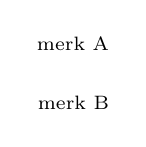
\begin{tikzpicture}[x=1.15cm,font=\scriptsize]
  \boxplot[.5]{1.3}{10.5}{11.3}{11.95}{12.55}{13.1} \node[left] at (7.8,1.3) {merk A};
  \boxplot[.5]{.55}{8.7}{10.0}{11.7}{14.0}{15.0} \node[left] at (7.8,.55) {merk B};
  \getalas[uur]{8}{1}{16}
\end{tikzpicture}}
\begin{stappenbreed}
\text{centrum: } \xbar_A \approx \xbar_B \approx 11,9 & De mediaan van A is iets hoger. Gemiddeld gaan ze even lang mee. \\
\text{spreiding: } \IKA_A = 1,25 \quad \IKA_B = 4 & De box van B is meer dan drie keer zo breed, en $s_B$ is bijna drie keer $s_A$. \\
\text{vorm: A vrij symmetrisch} & Bij B ligt de mediaan links in de box: de bovenste helft is breder.
\end{stappenbreed}
Gemiddeld houden beide merken het even lang vol, ongeveer 12 uur. Maar merk A is veel betrouwbaarder: elk toestel haalt minstens $10,5$ uur. Bij merk B haalt een kwart van de toestellen 14 uur of meer, maar een kwart haalt zelfs geen 10 uur. Wie zeker een volle dag wil, kiest merk A.}

\begin{werkwijze}
Teken de boxplots boven dezelfde getallenas. Vergelijk het centrum (mediaan of gemiddelde), de spreiding (interkwartielafstand, variatiebreedte of standaardafwijking) en de vorm (symmetrisch of scheef, uitschieters). Schrijf je besluit in volzinnen, in de context, met de getallen erbij.
\end{werkwijze}

\begin{oefeningen}
\oef{h3-boxplots}
\end{oefeningen}

\subsection{Aantallen of percentages?}

Op school A komen 180 leerlingen met de fiets, op school B 120. Fietsen er op school A dus meer leerlingen? In aantal wel. Maar als school A veel groter is, kan het aandeel fietsers er toch kleiner zijn. Groepen van verschillende grootte vergelijk je daarom met relatieve frequenties.

\voorbeeld{}{School A telt 600 leerlingen, waarvan 180 met de fiets komen. School B telt 300 leerlingen, waarvan 120 met de fiets komen. Op welke school fietsen relatief de meeste leerlingen?\label{vb:h3-relatief}}{%
\uitleg{De scholen zijn niet even groot. We berekenen voor elke school het percentage fietsers.}
\begin{stappen}
\text{school A: } \tfrac{180}{600} = 30~\% & Minder dan een derde. \\
\text{school B: } \tfrac{120}{300} = 40~\% & Tien procentpunt meer.
\end{stappen}
Op school A komen meer leerlingen met de fiets, maar op school B is het aandeel fietsers groter. Welke vergelijking je maakt, hangt af van de vraag: voor het aantal fietsenstallingen tel je, om te weten waar fietsen populairder is, vergelijk je percentages.}

Let ook op het verschil tussen \textit{procentpunt} en \textit{procent}. Van $30~\%$ naar $40~\%$ is een stijging met 10 procentpunt, maar het aandeel is met $\tfrac{10}{30} \approx 33~\%$ gestegen.

\begin{oefeningen}
\oef{h3-relatief}
\end{oefeningen}

\subsection{De juiste maat kiezen}

Gemiddelde of mediaan, standaardafwijking of interkwartielafstand: welke maten geef je? Uit de vorige delen weet je dat het gemiddelde en de standaardafwijking gevoelig zijn voor uitschieters en voor een lange staart, en de mediaan en de interkwartielafstand niet. Dat bepaalt de keuze.

\begin{werkwijze}
Is de verdeling ongeveer symmetrisch, zonder uitschieters, gebruik dan het gemiddelde en de standaardafwijking: die gebruiken alle gegevens. Is de verdeling scheef, of zijn er uitschieters, gebruik dan de mediaan en de interkwartielafstand. Bij kwalitatieve gegevens gebruik je de modus.
\end{werkwijze}

\voorbeeld{}{Bij de reactietijden van voorbeeld~\ref{vb:h3-uitschieter} wil een leerling in één zin zeggen hoe snel de groep reageert en hoe verschillend de leerlingen zijn. Welke maten kiest ze?\label{vb:h3-maatkiezen}}{%
\uitleg{Er is een uitschieter, 0,62 s. We kiezen maten die er weinig last van hebben.}
Ze kiest de mediaan en de interkwartielafstand: \textit{De helft van de leerlingen reageert sneller dan 0,31 s, en de middelste helft ligt binnen 0,04 s van elkaar.} Met het gemiddelde ($0,335$ s) en de standaardafwijking ($0,089$ s) zou het lijken alsof de groep trager en veel verschillender is dan ze is, door één afgeleide leerling.}

\begin{oefeningen}
\oef{h3-maat}
\end{oefeningen}

%========================================================================================
\section{Misleidende grafieken}

Een grafiek kan juiste getallen tonen en toch een verkeerde indruk geven. Soms is dat een vergissing, soms is het de bedoeling. Wie een grafiek leest, moet dus weten waar hij op moet letten. We bekijken de meest gebruikte trucs, te beginnen met het probleem.

\lkr{Laat leerlingen een misleidende grafiek uit een krant, een reclame of sociale media meebrengen, en bespreek ze met de werkwijze om een grafiek kritisch te lezen. Opdracht~\ref{oef:h3-o20}, waarin ze zelf een misleidende en een eerlijke grafiek maken, kan een groepsopdracht worden.}

\subsection{Een as die niet bij 0 begint}

In een staafdiagram vergelijk je de lengte van de staven. Begint de verticale as niet bij 0, dan zijn de lengtes niet meer evenredig met de getallen: een klein verschil lijkt groot.

\voorbeeld{}{Terug naar het probleem. Hoeveel keer zo hoog lijkt de staaf van 2024 in grafiek 1 als die van 2019? Hoeveel is het aantal fietsers echt gestegen? Wie heeft gelijk?\label{vb:h3-terug}}{%
\uitleg{In grafiek 1 begint de as bij 1800. We vergelijken de lengte van de staven met de echte getallen.}
\begin{stappenbreed}
\text{grafiek 1: } \dfrac{1960 - 1800}{1820 - 1800} = \dfrac{160}{20} = 8 & De staaf van 2024 is 8 keer zo lang. \\[2ex]
\text{echt: } \dfrac{1960}{1820} \approx 1,077 & Het aantal is $7,7~\%$ gestegen. \\[1.5ex]
1960 - 1820 = 140 & 140 fietsers per dag meer.
\end{stappenbreed}
Beide grafieken tonen de juiste getallen, maar grafiek 1 laat een stijging van $7,7~\%$ lijken op een verachtvoudiging. Die grafiek misleidt. Grafiek 2 begint bij 0 en toont de verhoudingen eerlijk, maar \textit{nauwelijks veranderd} is ook overdreven: 140 fietsers per dag meer, elk jaar wat meer, is een duidelijke en gestage stijging. Een eerlijk besluit: \textit{Het aantal fietsers steeg in vijf jaar met ongeveer $8~\%$.}}

Mag een as dan nooit bij een ander getal dan 0 beginnen? Bij een lijndiagram, waar je het verloop wilt zien, mag dat wel, als je het duidelijk aangeeft met een zigzag op de as. Bij een staafdiagram, waar je lengtes vergelijkt, begint de as altijd bij 0.

\begin{oefeningen}
\oef{h3-as}
\end{oefeningen}

\subsection{Oppervlakte en pictogrammen}

Een krant wil tonen dat het zakgeld van jongeren verdubbeld is. In plaats van staven tekent ze een spaarvarken, en voor het nieuwe zakgeld een spaarvarken dat twee keer zo hoog is. Maar een tekening die twee keer zo hoog is, is ook twee keer zo breed. Wat zie je dan?

\voorbeeld{}{Het zakgeld steeg van 20 naar 40 euro. In een grafiek wordt dat getekend als een vierkant met zijde 1 cm en een vierkant met zijde 2 cm. Hoeveel keer zo groot lijkt het nieuwe zakgeld?\label{vb:h3-pictogram}}{%
\uitleg{Het oog vergelijkt oppervlaktes, niet hoogtes. We berekenen de oppervlakte van beide vierkanten.}
\naast{\begin{stappenvrij}{4.6cm}{4.6cm}
1 \cdot 1 = 1 \text{ cm}^2 & Het oude zakgeld. \\
2 \cdot 2 = 4 \text{ cm}^2 & Het nieuwe: vier keer zo groot.
\end{stappenvrij}
\vspace{1mm}
{\itshape Het zakgeld is verdubbeld, maar het lijkt vervierdvoudigd. Eerlijk is: twee vierkanten even breed, het ene twee keer zo hoog, of gewoon twee staven.}}{\begin{tikzpicture}[font=\scriptsize]
  \fill[accent!35] (0,0) rectangle (1,1); \draw[accent] (0,0) rectangle (1,1); \node[below] at (.5,0) {20 euro};
  \fill[accent!35] (1.6,0) rectangle (3.6,2); \draw[accent] (1.6,0) rectangle (3.6,2); \node[below] at (2.6,0) {40 euro};
\end{tikzpicture}}}

Bij een tekening die diepte suggereert, zoals een driedimensionale munt of ton, is het nog erger: twee keer zo hoog, breed en diep is acht keer zo groot.

\begin{oefeningen}
\oef{h3-pictogram}
\end{oefeningen}

\subsection{Een ongelijke schaal en een gekozen periode}

Ook de horizontale as kan misleiden. Staan de jaartallen op gelijke afstand terwijl de tijd ertussen verschilt, dan lijkt een verloop sneller of trager dan het is. En wie zelf kiest welke periode hij toont, kan een stijging of een daling laten zien naar keuze.

\voorbeeld{}{Een sportclub toont haar ledenaantal op een lijndiagram, met de jaren op gelijke afstand (links): 2000: 120, 2010: 160, 2020: 200, 2022: 240, 2024: 280. Het bestuur schrijft: \textit{We groeien al jaren even snel.} Klopt dat?\label{vb:h3-schaal}}{%
\uitleg{Op het diagram van de club is de lijn een rechte. Maar tussen de eerste jaartallen zitten tien jaar, tussen de laatste maar twee. We berekenen de groei per jaar.}
\begin{stappenbreed}
2000 \to 2010\text{: } \tfrac{160 - 120}{10} = 4 & 4 leden per jaar. \\
2010 \to 2020\text{: } \tfrac{200 - 160}{10} = 4 & 4 leden per jaar. \\
2020 \to 2022\text{: } \tfrac{240 - 200}{2} = 20 & 20 leden per jaar. \\
2022 \to 2024\text{: } \tfrac{280 - 240}{2} = 20 & 20 leden per jaar.
\end{stappenbreed}
\figuren{\begin{tikzpicture}[x=.9cm,y=.01cm,font=\scriptsize]
  \frequentieas[leden]{100}{300}{-.4}{4.4}
  \foreach \j/\l [count=\i from 0] in {2000/120,2010/160,2020/200,2022/240,2024/280}{\fill[accent] (\i,\l) circle (2pt); \node[below] at (\i,0) {\j};}
  \draw[accent,thick] (0,120) -- (4,280);
  \node at (2,-70) {met de jaren op gelijke afstand};
\end{tikzpicture}\qquad\qquad
\begin{tikzpicture}[x=.16cm,y=.01cm,font=\scriptsize]
  \frequentieas[leden]{100}{300}{-1}{25}
  \foreach \j/\l in {0/120,10/160,20/200,22/240,24/280}{\fill[accent] (\j,\l) circle (2pt);}
  \draw[accent,thick] (0,120) -- (10,160) -- (20,200) -- (22,240) -- (24,280);
  \foreach \j in {0,10,20}{\pgfmathtruncatemacro{\a}{2000+\j}\node[below] at (\j,0) {\a};}
  \node[below,anchor=north west,xshift=-1mm] at (24,0) {2024};
  \node at (12,-70) {met een eerlijke tijdas};
\end{tikzpicture}}
Met een eerlijke tijdas (rechts) zie je dat de club sinds 2020 vijf keer zo snel groeit als ervoor. Het bestuur heeft dus geen gelijk: de groei versnelt sterk.}

\begin{oefeningen}
\needspace{12\baselineskip}
\oef{h3-schaal}
\end{oefeningen}

\subsection{Kritisch lezen}

Er zijn nog meer manieren om met een grafiek of een getal te misleiden: een cirkeldiagram waarvan de delen samen geen $100~\%$ zijn, een grafiek zonder eenheden, een percentage zonder het aantal waarop het berekend is, of een gemiddelde waar een mediaan beter zou passen. Een korte reeks vragen helpt je om ze te ontmaskeren.

\begin{werkwijze}
Een grafiek kritisch lezen: lees de titel, de assen en de eenheden. Begint de verticale as bij 0, en is de schaal gelijkmatig? Zijn het aantallen of percentages, en hoeveel gegevens zijn er? Welke periode zie je, en wat zou je zien met een langere periode? Past de maat bij de gegevens? Formuleer daarna zelf een eerlijk besluit.
\end{werkwijze}

\voorbeeld{}{Een fabrikant van tandpasta adverteert: \textit{8 op 10 tandartsen raden ons merk aan!} In de kleine letters staat dat 10 tandartsen ondervraagd werden, en dat ze meerdere merken mochten aanduiden. Wat vind je van de reclame?\label{vb:h3-kritisch}}{%
\uitleg{We gaan na hoeveel gegevens er zijn, en wat de vraag precies was.}
Er werden maar 10 tandartsen ondervraagd: met zo weinig gegevens kan het toeval een grote rol spelen. Bovendien mochten ze meerdere merken aanduiden: het kan best dat 8 op 10 tandartsen ook elk ander merk aanraden. De reclame zegt dus niet dat tandartsen dit merk verkiezen boven andere. Een eerlijk besluit: \textit{In een kleine groep van 10 tandartsen noemden er 8 dit merk als een van de merken die ze aanraden.}}

\begin{oefeningen}
\oef{h3-kritisch}
\end{oefeningen}

%========================================================================================
\opdrachtenkop

\begin{oefeningen}
\oef{h3-o1}

\oef{h3-o2}

\oef{h3-o3}

\oef{h3-o4}

\oef{h3-o5}

\needspace{12\baselineskip}
\oef{h3-o6}

\oef{h3-o7}

\oef{h3-o8}

\oef{h3-o9}

\oef{h3-o10}

\oef{h3-o11}

\oef{h3-o12}

\oef{h3-o13}

\oef{h3-o14}

\oef{h3-o15}

\oef{h3-o16}

\oef{h3-o17}

\oef{h3-o18}

\needspace{12\baselineskip}
\oef{h3-o19}

\oef{h3-o20}

\oef{h3-o21}

\oef{h3-o22}
\end{oefeningen}

%----------------------------------------------------------------------------------------
\opdrachtsectie{Test jezelf}

\begin{oefeningen}
\oef{h3-t1}

\oef{h3-t2}

\oef{h3-t3}

\oef{h3-t4}

\oef{h3-t5}

\oef{h3-t6}

\oef{h3-t7}
\end{oefeningen}

\herhaalschema{%
  \fv{oef:h3-t1}{vb:h3-vorm}{oef:h3-vorm}%
  \fv{oef:h3-t2}{vb:h3-gemmed}{oef:h3-gemmed}%
  \alleenvoor{1,2,3}{\fv{oef:h3-t3}{vb:h3-uitschieter}{oef:h3-uitschieter}}\alleenvoor{4,5}{\fv{oef:h3-t3}{vb:h3-regel}{oef:h3-uitschieter}}%
  \fv{oef:h3-t4}{vb:h3-boxplots}{oef:h3-boxplots}%
  \fv{oef:h3-t5}{vb:h3-relatief}{oef:h3-relatief}%
  \fv{oef:h3-t6}{vb:h3-terug}{oef:h3-as}%
  \fv{oef:h3-t7}{vb:h3-pictogram}{oef:h3-pictogram}}

\ifzelfstudie
\section*{Maak je eigen samenvatting}
Sluit dit boek en schrijf in je schrift: wat een symmetrische, rechtsscheve en linksscheve verdeling is, hoe het gemiddelde en de mediaan dan liggen, wat een uitschieter met de maten doet, hoe je twee groepen vergelijkt, wanneer je percentages gebruikt, welke maten je kiest bij welke gegevens, en de vragen om een grafiek kritisch te lezen. Vergelijk daarna met de kaders.
\fi
